\section{Progettazione}
\begin{frame}{Suddivisione architetturale}
\begin{itemize}
  \item package \texttt{constraintobj}
  \item package \texttt{solver}
  \item package \texttt{gui}
\end{itemize}
\end{frame}

\begin{frame}{Rappresentazione dei domini}


class Domain
\begin{itemize}
  \item[-] accepted: Set[String]
  \item[+] contains(elem: String): Boolean
\end{itemize}
\end{frame}

\begin{frame}{Rappresentazione dei vincoli}
class Constraint
\begin{itemize}
  \item[-] vars: Array[String]
  \item[-] accepted: List[Array[String]]
  \item[+] projection(variable: String): Set[String]
  \item[+] reduction(variable: String, value: String): Constraint
\end{itemize}
\end{frame}

\begin{frame}[fragile]{Esempio di oggetto constraint}
\begin{verbatim}
c = Constraint(vars     =>  [X, Y, Z]
               accepted => [[0, 0, 1],
                            [0, 1, 1],
                            [0, 1, 0]])
                            
c.projection(X) = [0]
c.projection(Y) = [0, 1]

c.reduction(Y,1) = Constraint(vars     =>  [X, Y, Z]
                              accepted => [[0, 1, 1],
                                           [0, 1, 0]])
\end{verbatim}  
\end{frame}

\begin{frame}{Rappresentazione degli ordini - 1}
\begin{itemize}
  \item class Order
  \item \textbf{Rappresentazione ad albero}: nodi interni per gli assegnamenti, foglie per gli ordini
  \pause
  \item class Comparator per l'accesso
  \item Complessità dipendente dalla \textbf{ricerca nei nodi interni}
  \begin{itemize}
  	\item Ricerca lineare: $O(|dom(V_1)|+\ldots+|dom(V_n)|)$
  	\item Ricerca binaria: $O(log(|dom(V_1)|\cdot \ldots \cdot|dom(V_n)|))$
  	\item Tabella hash:    $O(1)$
  \end{itemize}
\end{itemize}
\end{frame}

\begin{frame}{Rappresentazione degli ordini - 2}
Esempio

\texttt{var A dependsON=\{B,C,D\}}  \texttt{dom=\{...\}}\\
\texttt{var B dependsON=\{\}}       \texttt{dom=\{$b$,$\overline{b}$\}}\\
\texttt{var C dependsON=\{\}}       \texttt{dom=\{$c$,$\overline{c}$\}}\\
\texttt{var D dependsON=\{\}}       \texttt{dom=\{$d$,$\overline{d}$\}}\\
\begin{center}
  \begin{figure}[ht]
    \centering
    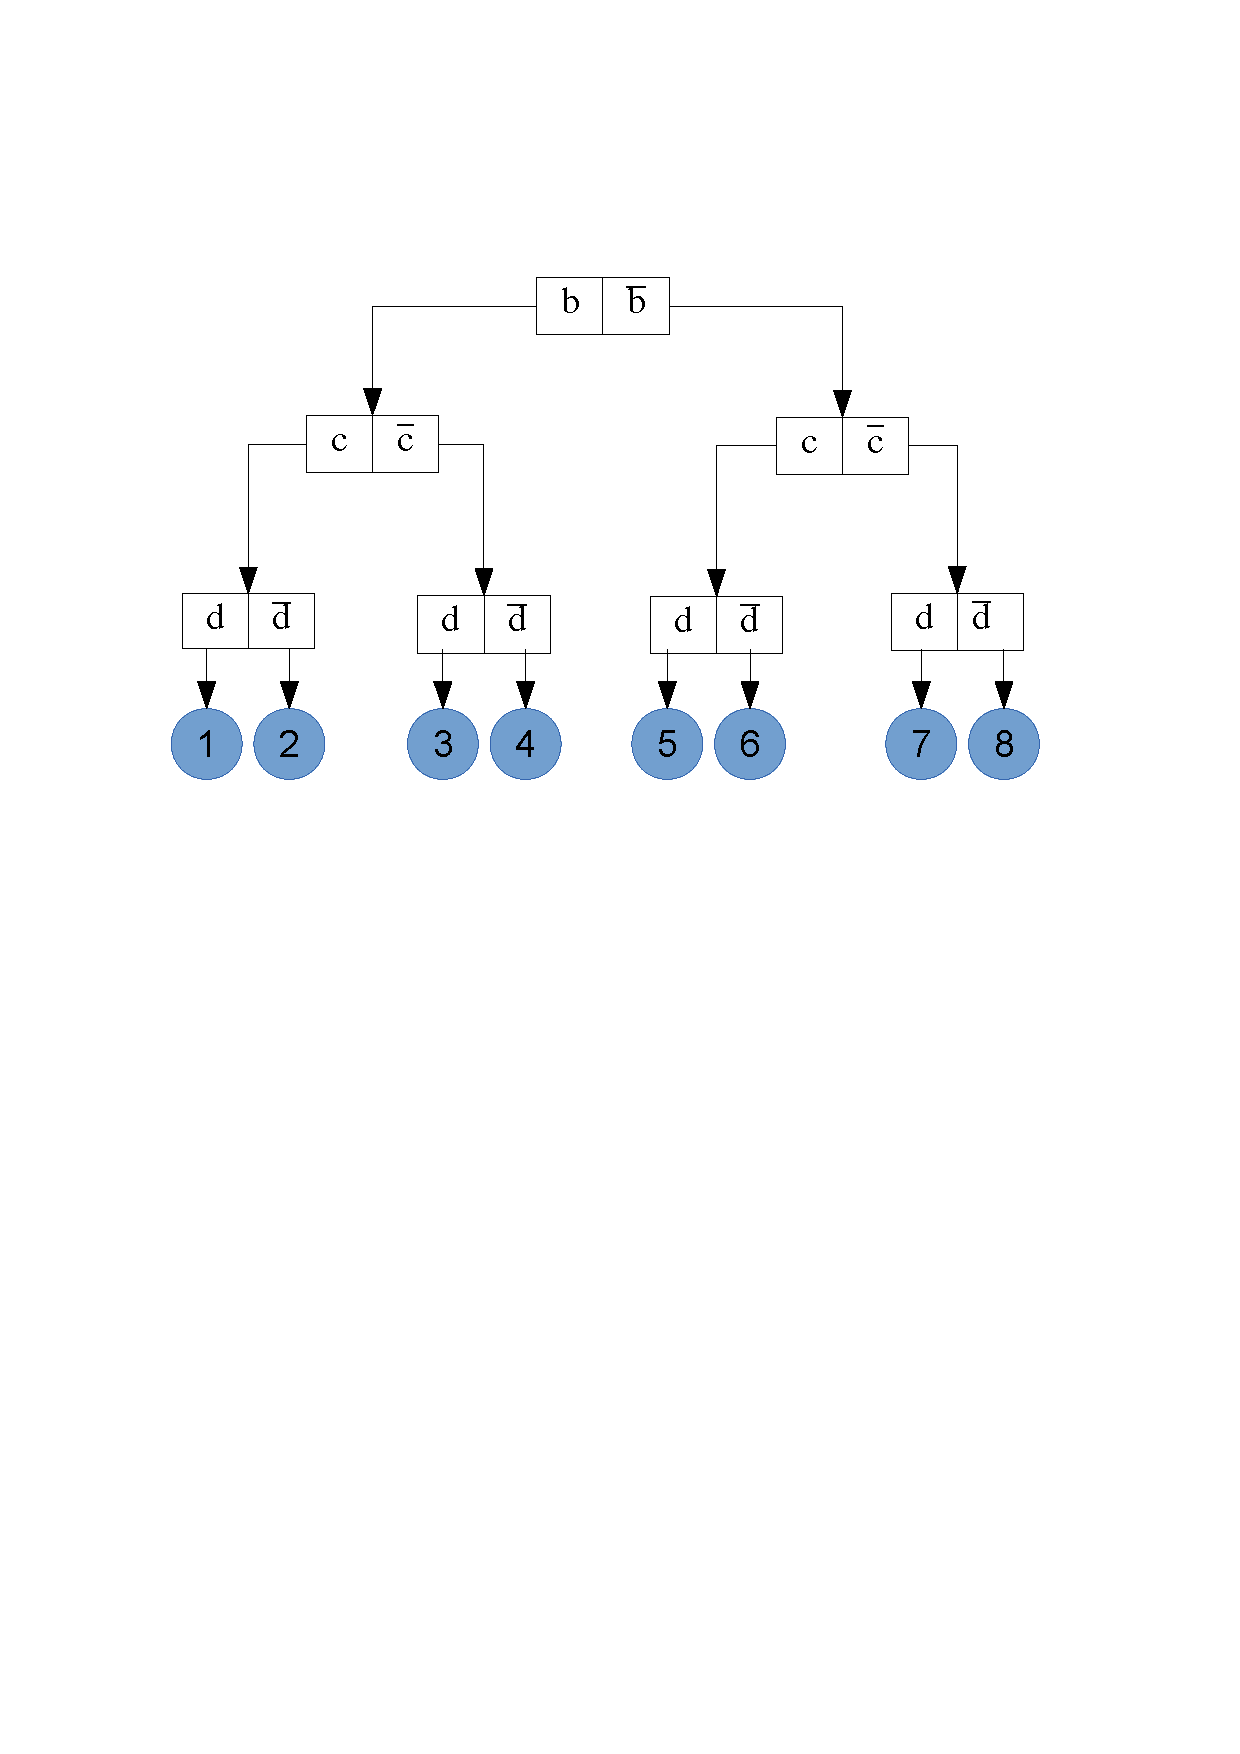
\includegraphics[width=0.5\textwidth]{grafo-ordini}
    \caption{\textit{Rappresentazione a grafo di A, B, C, D}}
  \end{figure}
\end{center}
\end{frame}